% Software
\specialsection{Software}{}{black}{white}

\begin{figure}
  \centering
  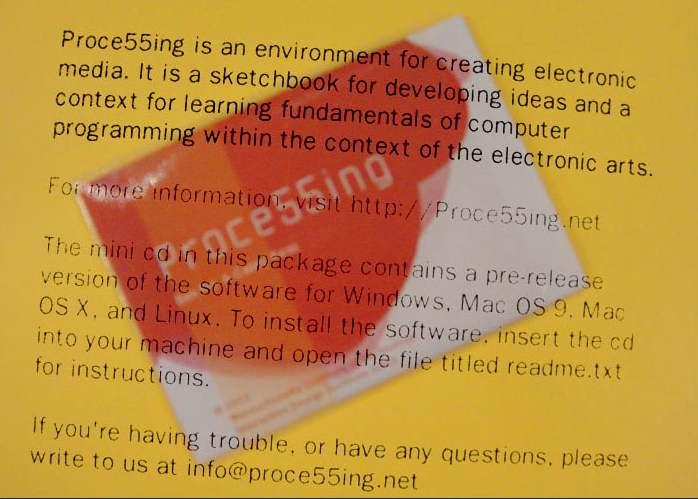
\includegraphics[width=0.9\textwidth]{images/processing-mini-cd.png} 
  \caption{Mini CDs for sponsors at the Media Lab Open House october 2002}
  \label{fig:processing-cd}
\end{figure}
\subsection{Release early, release often}
The maxim "Release early, release often," attributed to Eric S. Raymond in his seminal text "The Cathedral and the Bazaar" \parencite{raymondCathedralBazaar1999}, is often touted as a catalyst for vibrant open-source communities. In particular, projects like Linux have benefited from this approach, allowing rapid integration of contributions from a distributed network of contributors. This not only boosts the morale of individual contributors but also creates a dynamic and responsive development environment.

However, the Processing project presents a departure from this pattern. The time-between-releases data, presented in the table below, reveals periods of intense activity interlaced with long intervals of inactivity, complicating a straightforward mapping onto the “Release early, release often” model.

\changepapersize{305.3mm:210mm}
\customtag{largepage}

{
\LARGE
\noindent Frequency of Releases\par
\vspace{0.2cm} % Adjust the 1cm to the amount of vertical space you want
}


\begin{multicols}{3}
  \noindent
  \begin{minipage}{\columnwidth + \columnsep}    
      \begin{tabular}{|r|l|}
        \hline
        Descriptive statistics & Time between releases \\
        \hline
        count & 60 \\
        mean & 20 days 15:11 \\
        std & 47 days 00:10 \\
        min & 0 days 00:00 \\
        25\% & 1 days 00:00 \\
        50\% & 3 days 00:00 \\
        75\% & 26 days 18:00 \\
        max & 338 days 00:00 \\
        \hline
      \end{tabular}
      \captionof{table}{Release statistics}
  \end{minipage}
  
  \columnbreak % Force break to the next column
  
  % The second minipage will span one column (1/3 of the text width)
  \noindent
  \begin{minipage}{\columnwidth}
    \frame{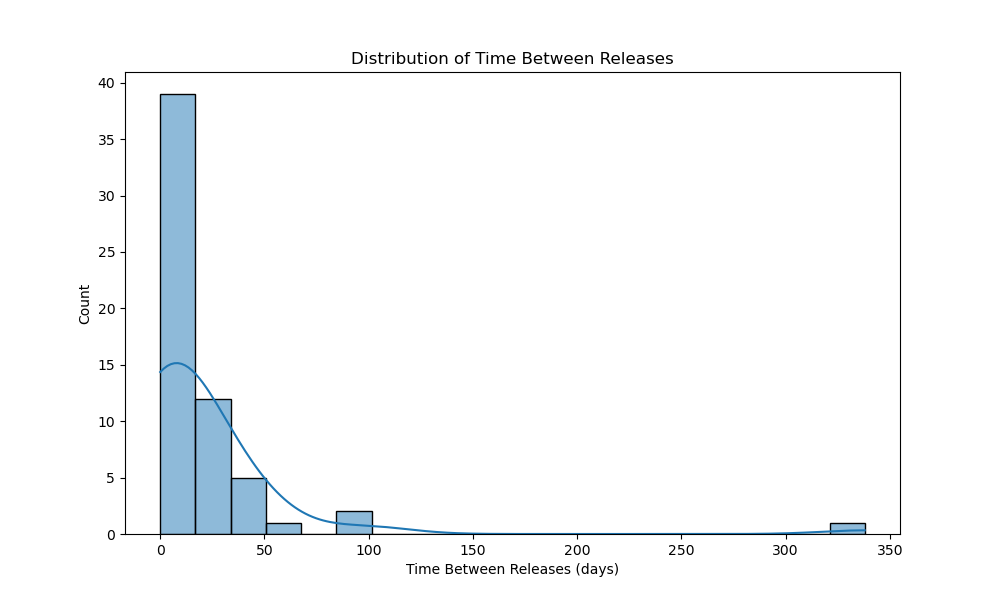
\includegraphics[width=\linewidth]{images/time_between_releases_histogram.png}}
      % \includegraphics[width=\linewidth]{graph2}
      \captionof{figure}{Graph that spans one column}
  \end{minipage}
  
  % Any text after this will continue in a three-column layout
  \end{multicols}
  
\begin{figure}[h!] 
  \centering
  \frame{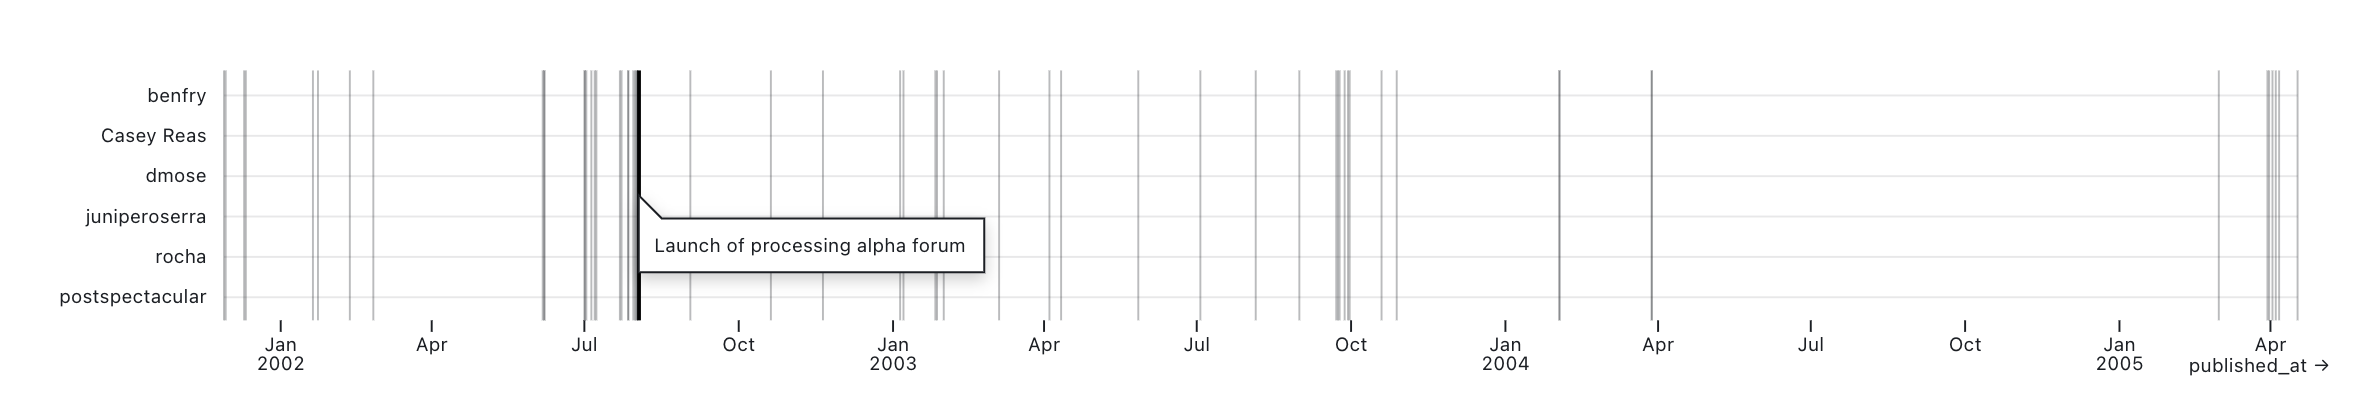
\includegraphics[width=1\textwidth]{images/releases-lines.png}}
  \caption{Time between releases}
  \label{fig:releases-lines}
\end{figure}

% \begin{figure}[h!] 
%   \centering
%   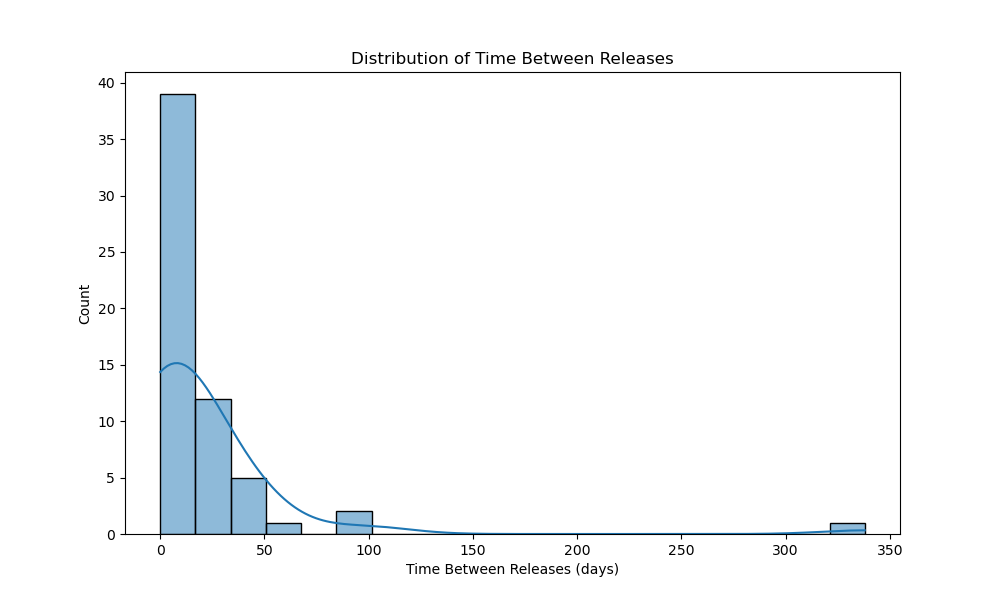
\includegraphics[width=0.9\textwidth]{images/time_between_releases_histogram.png} 
%   \caption{Time between releases histogram}
%   \label{fig:releases_frequency_histogram}
% \end{figure}

\begin{multicols}{3}
  \noindent
  The graphical representations depict a distinctive pattern of release clustering, a testament to the sporadic and intermittent nature of the project's development lifecycle. A notable surge can be observed leading up to pivotal milestones, such as the alpha forum's initial release, indicating a focused burst of activity during these critical junctures.
  \noindent
The distribution of releases further accentuates the project's non-linear progress, with a marked increase in releases as key points approach, followed by periods of relative inactivity. This ebb and flow suggest that the development process is influenced by external factors or revolves around specific events, leading to a "feast or famine" scenario in terms of updates and improvements.
\noindent
Moreover, the extended intervals devoid of any releases could imply that the project advancement is perhaps a secondary or parallel endeavor for the contributors. 
\end{multicols}

\defaultareasettings

What makes Processing a particularly interesting case is that, contrary to what one might expect from Raymond's model, most contributions appear to be made by a centralized figure—Ben Fry, the project's main architect—rather than a broad community of external contributors. This effectively shifts the project's development model closer to a cathedral-like structure for core components, as reflected by Ben's direct control over major releases. 

Moreover, the project’s side-project nature is confirmed by revision comments such as one from 05/01/2003, which reads: "hopefully January 2003 will be a good month for p5, as I have a short bit of time to work on it [...] I hope to get a few revisions out this month so I can get back to my 'real' work." These comments illuminate that, for core contributors, Processing is not necessarily viewed as a full-time commitment.

The perception of Processing as a side project rather than a full-time commitment for its core contributors is corroborated through multiple channels. For example, a revision comment from May 1, 2003, highlights this sentiment, stating, ``hopefully January 2003 will be a good month for p5, as I have a short bit of time to work on it [...] I hope to get a few revisions out this month so I can get back to my `real' work.'' This observation is further substantiated by a 2021 study titled ``Graphic design in the post-digital age: a survey of practices fueled by creative coding,'' which notes that Processing began as a personal initiative and was largely developed during nights and weekends. The study further reveals that the project received indirect funding from MIT through Fry's graduate stipend, and from Interaction Design Institute Ivrea (IDII) through Reas's salary, again indicating its ancillary nature in the professional lives of its principal contributors~\parencite[396]{conradGraphicDesignPostdigital2021}.

It is worth noting that the logistics of releasing software were more complex in the early 2000s than they are today. As can be seen in Figure~\ref{fig:processing-cd} of a mini CD from October 2002 illustrates, distributing software was not as straightforward as pushing updates to a Git repository.



% Trends in git commits
The \textit{Processing} project illuminates a crucial challenge often faced by open source communities: the dependency on key contributors. In the case of Processing, Ben Fry's central role over the past two decades raises concerns about the project's resilience and sustainability. His substantial contributions create a high-risk situation termed the "bus factor" \parencite{BusFactor2023}, which indicates how vulnerable a project becomes when overly reliant on a single or a small number of contributors. This vulnerability is not unique to Processing, as such dependency models are commonly observed across open source projects, often humorously discussed in popular culture \parencite{munroeDependency2020}.

The imbalanced contribution landscape is vividly illustrated in Figure~\ref{fig:alpha-commits}. During the period of the alpha forum, only six individuals contributed code to the repository. This stands in stark contrast to the activity on the forum, where over 1000 individuals were engaged in discussions and queries. The commits themselves were also sporadic and infrequent. As Casey aptly points out: ``I think one thing that’s important to clarify is that Ben Fry, my collaborator, is the primary software engineer of the project [...]'' \parencite[p. 330]{conradGraphicDesignPostdigital2021}.

\begin{figure}[h!] 
  \centering 
  \includesvg[pretex=\sffamily\fontsize{5.58pt}{8pt}\selectfont, width=1\textwidth, keepaspectratio]{images/processing-alpha-commits.svg}
  \caption{Commits up to and including the Processing alpha forum}
  \label{fig:alpha-commits}  
\end{figure}

This discrepancy between the number of code contributors and forum participants is indeed profound, as corroborated by the subsequent visualizations ~\ref{fig:top12-github} and comic anecdotes ~\ref{fig:dependency_comic}. The limited number of contributors to the codebase and the concentrated responsibility on a few individuals amplify the bus factor risk, an issue that warrants deeper investigation and consideration for the long-term health of the project.


\begin{figure}[h!] 
    \centering 
    \includesvg[pretex=\sffamily\fontsize{5.58pt}{8pt}\selectfont, width=1\textwidth, keepaspectratio]{images/figure-top12-github.svg}
    \caption{Top 12 source code contributors by number of commits}
    \label{fig:top12-github}  
  \end{figure}

\begin{figure}[h!] 
    \centering
    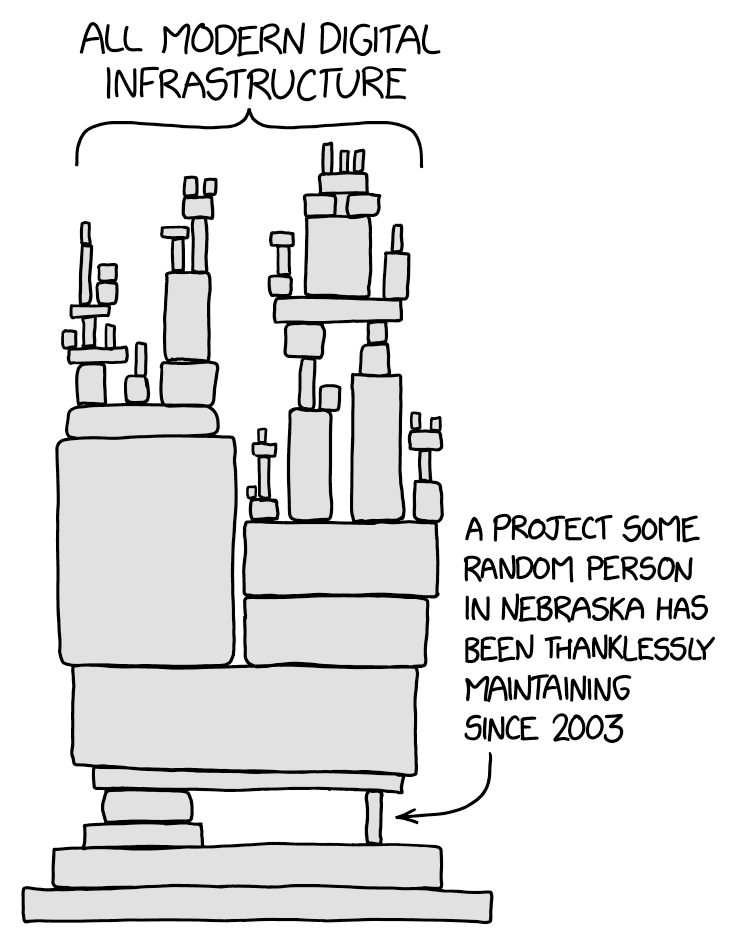
\includegraphics[width=0.5\textwidth]{dependency.png} 
    \caption{Dependency}
    \label{fig:dependency_comic}
    \small Source: \textit{XKCD}, \url{https://xkcd.com/2347/}, licensed under CC BY-NC 2.5.
\end{figure}

The commit logs within the Processing project's GitHub repository, while rich with data, do not provide a complete visualization of early contributions. In an interview with Ben Fry, it was elucidated that contributions from various lab members, including those from Simon Greenwold, were indeed substantial in the project's formative years. These contributions, although crucial, are not conspicuously traceable through the GitHub interface. Fry explains that due to the constraints of the version control systems like CVS and Subversion used at the time, he personally committed code from other contributors, ensuring their efforts were acknowledged in the commit logs, even if not directly attributed in the repository's graphical interface.

Moreover, Fry sheds light on the complex interplay between the Processing project and MIT's evolving stance towards open source software. He recounts the early difficulties: "We also had a long delay before we could release the code publicly, because we got stuck in a period when MIT, and the Media Lab in particular, were figuring out its relationship to open source code. The TLO was suddenly taking an interest in all these things that were simply being given away as ‘open source,’ so it took us a couple years to get actual clearance for it." This statement points to the broader challenges faced by academic institutions in reconciling their intellectual property policies with the principles of the open source movement, a context that is vital for understanding the trajectory of Processing's development and distribution.

\subsection{A cathedral or a bazaar}

While existing literature often focuses on the role of companies in contributing to open-source projects through complementary services like consulting, our study diverges by focusing on individual contributors. In the context of the Processing community, corporate involvement is notably lesser when compared to platforms like Linux that have substantial corporate contributions.

The 2016 Processing community survey revealed a significant number of users employ the language for educational purposes. This is consistent with Processing's design ethos, which is aimed at being educationally accessible. However, the extent to which this educational usage intersects with what can be termed as `professional use' remains unclear.

For the purpose of this study, `professional use' is understood to primarily include artists and designers. This nuanced categorization helps in probing the overlap between professional and educational use within the Processing community.

Building upon established frameworks such as the taxonomy by Bonaccorsi et al.~\cite{bonaccorsiComparingMotivationsIndividual2006}, which categorizes motivations behind open-source contributions into Economic, Social, and Technological domains, our study intends to adapt this taxonomy to suit the specific nuances of the Processing community.

\begin{figure}[h!] 
  \centering
  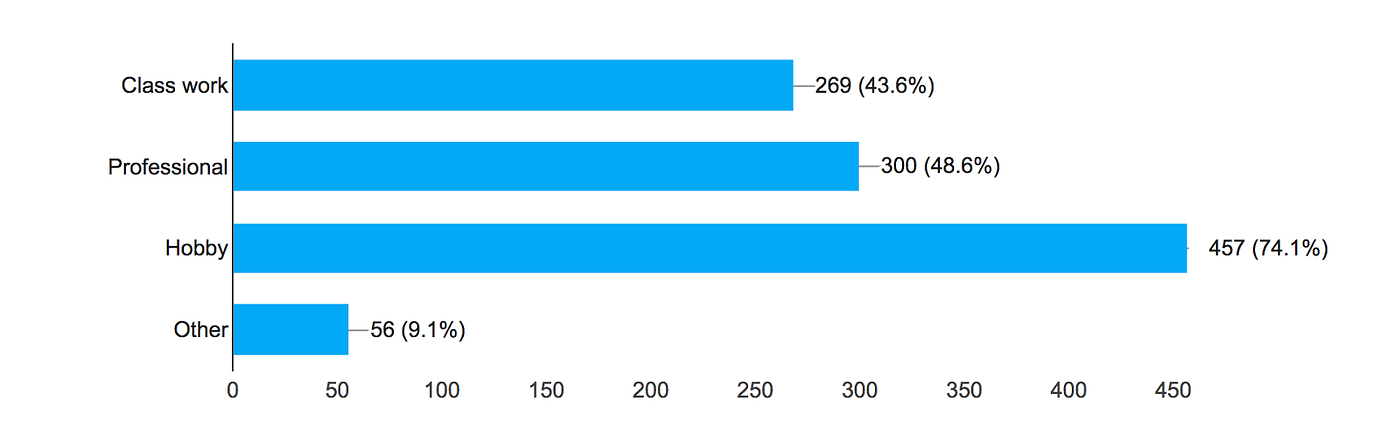
\includegraphics[width=0.9\textwidth]{images/community-survey.png} 
  \caption{Processing 2016 community survey result \parencite{2016CommunitySurvey}}
  \label{fig:community_survey}
\end{figure}

\begin{table}
    \begin{tabularx}{\textwidth}{l X} % X is a placeholder for stretching the column
    \toprule
    Motivation area & Micro level \\
    \midrule
    Economic & Monetary rewards \\
     & Low opportunity costs \\
     & Gaining a reputation among peers \\
     & Gaining future career benefits \\
    \midrule
    Social & Fun to program (Loving to code) \\
     & Altruism (gift economy) \\
     & Sense of belonging to the community \\
     & Fight against proprietary software \\
    \midrule
    Technological & Learning \\
     & Contributions and feedback from the community \\
     & Working with a bleeding-edge technology \\
     & Scratching a personal itch \\
    \bottomrule
    \end{tabularx} % End of tabularx environment
    \label{tab:taxonomy}
    \caption{Taxonomy of Individual Programmers’ Motivations. Adapted from \parencite{bonaccorsiComparingMotivationsIndividual2006}}

\end{table}

% todo NN cette taxonomie est intéressante, mais il faudrait la commenter dans le corps de texte en 2.2, qu’elle vienne nourrir ce que tu as mis au-dessus comme texte, là tu la pose rapidement sans trop détailler comment elle a été produite et ce qu’elle nous dit

%\subsection{The intersection of Creative Coding and Open Source}
%\subsection{Relevant Methodological Approaches in Computer Science and Anthropology}

\subsection{Open Source Contributions}

Open source software has evolved from a grassroots, community-driven activity into a mainstream phenomenon influencing all sectors of software development. This transition has been analyzed from numerous perspectives, including Etienne Wenger's theory of Communities of Practice, which posits that learning occurs in social contexts \parencite{wengerCommunitiesPracticeLearning1998}. This theory underscores the importance of shared experiences, tools, and discourse in shaping a community's collective practice. In the context of open-source software, these dynamics offer invaluable insights into the sustainability and progression of such projects. For instance, the Processing community exemplifies more than just a collection of individual contributors; it represents a dynamic community molded by common goals and collective learning.

This communal focus contrasts sharply with the software development models described in Eric S. Raymond's seminal work "The Cathedral and the Bazaar" \parencite{CathedralBazaarMusings2002a}. The Cathedral model is marked by careful planning and centralized authority, more akin to the early GNU projects initiated by Richard Stallman in the 1980s. Conversely, the Bazaar model encourages open collaboration and decentralization—features commonly associated with contemporary open source projects. These two models can be conceptualized as endpoints of a continuum, with real-world communities of practice, like the Processing community, potentially embodying characteristics of both.

Although Richard Stallman's Free Software Movement initially utilized a Cathedral-like approach, the evolution of version control systems like Git has facilitated the adoption of more decentralized, Bazaar-like models. This technological and philosophical shift intriguingly complements Wenger's notions of "mutual engagement," "joint enterprise," and "shared repertoire"—elements that nurture a sense of community and shared objectives \parencite{wengerCommunitiesPracticeLearning1998}.

Fast-forwarding to today, the landscape now includes not just individual contributors but major corporations as well, injecting both challenges and opportunities into existing communities. The Processing project stands as a compelling case study to examine how an open-source community can preserve its foundational ethos while simultaneously adapting to contemporary requirements.

To holistically grasp the intricate interplay of social and technical factors contributing to the success of open-source initiatives, a multidimensional analysis is essential. Such an approach would synthesize various frameworks, including Wenger's Communities of Practice \parencite{wengerCommunitiesPracticeLearning1998} and Raymond's Cathedral and Bazaar models \parencite{CathedralBazaarMusings2002a}, aiming to provide a nuanced understanding of a community's past, present dynamics, and future potential.

